\chapter{AGES III}

\section{Introdução}

A dificuldade de entender, organizar e melhorar a própria vida
financeira é uma dor muito comum no Brasil. Muitos brasileiros chegam ao
fim do mês sem saber exatamente para onde o dinheiro foi --- não por
falta de interesse, mas porque nunca foram ensinados, de forma simples e
prática, a cuidar do próprio dinheiro. Diante desse cenário, surgiu a
proposta do FinUp: um aplicativo mobile que funciona como um "copiloto
financeiro do brasileiro", ajudando o usuário a controlar seus gastos,
tomar melhores decisões no dia a dia e aprender finanças de forma leve,
gamificada e sem julgamento.

A solução une organização financeira, inteligência artificial e educação
financeira em uma experiência acessível, jovem e prática. Entre suas
principais funcionalidades estão o controle de receitas e despesas, um
diagnóstico financeiro inicial, um indicador de saúde financeira (FinUp
Score), um assistente de IA para orientação no cotidiano, trilhas de
educação financeira gamificadas e um painel administrativo web.

Mais do que uma ferramenta de controle de gastos, o FinUp representa uma
iniciativa de impacto social, buscando democratizar o acesso à educação
financeira e empoderar seus usuários para que construam uma relação mais
saudável e consciente com o próprio dinheiro.

\section{Desenvolvimento do Projeto}

\textbf{Stakeholders do Projeto:}

\begin{itemize}
\item
  Vitor Oppermann
\item
  Diogo Ninov
\end{itemize}

\textbf{Período de Execução}: Segundo semestre de 2026.

\textbf{Professor Orientador:} Afonso Sales

\begin{figure}[htbp]
  \centering
  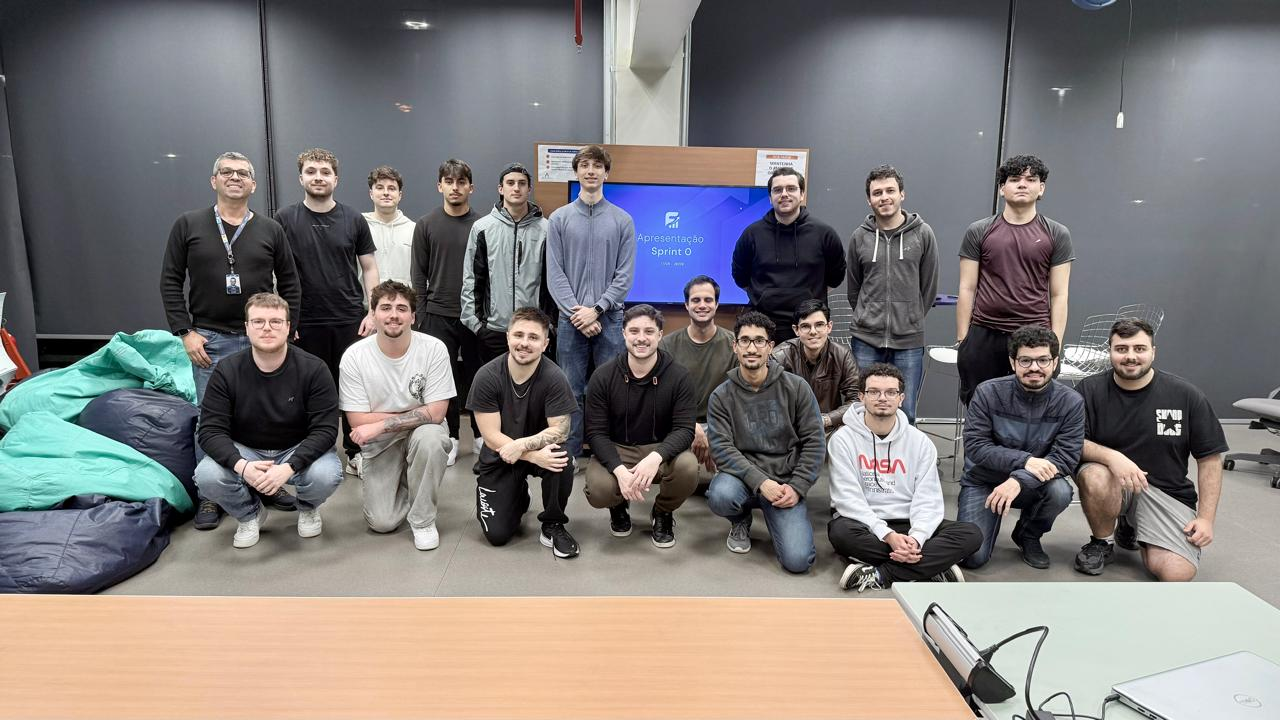
\includegraphics[width=\textwidth]{imagens/equipe-finup.jpeg}
  \caption{Equipe do projeto FinUp}
  \label{fig:equipe-finup}
\end{figure}

\begin{enumerate}
\def\labelenumi{\arabic{enumi}.}
\item
  \textbf{Repositório do código Fonte do Projeto}
\end{enumerate}

Wiki: \url{https://tools.ages.pucrs.br/2026-2/6lmnp/finup/finup-wiki}

Frontend Web:
\url{https://tools.ages.pucrs.br/2026-2/6lmnp/finup/finup-web}

Frontend Mobile:
\url{https://tools.ages.pucrs.br/2026-2/6lmnp/finup/finup-mobile}

Backend:
\url{https://tools.ages.pucrs.br/2026-2/6lmnp/finup/finup-backend}

\begin{enumerate}
\def\labelenumi{\arabic{enumi}.}
\setcounter{enumi}{1}
\item
  \textbf{Banco de Dados utilizado}
\end{enumerate}

\begin{quote}
Link para a wiki do banco:
\url{https://tools.ages.pucrs.br/2026-2/6lmnp/finup/finup-wiki/-/wikis/Banco\%20de\%20Dados}

O banco de dados do FinUp utiliza o modelo relacional, organizado em
três domínios: perfil do usuário, controle financeiro e educação
financeira gamificada . A escolha se justifica pela natureza estruturada
e interligada dos dados, garantindo integridade e consistência por meio
de chaves primárias e estrangeiras. As convenções adotadas incluem
nomenclatura em inglês com PascalCase e campos de auditoria, assegurando
padronização e facilitando a evolução do banco.
\end{quote}

\begin{enumerate}
\def\labelenumi{\arabic{enumi}.}
\setcounter{enumi}{2}
\item
  \textbf{Arquitetura utilizada}
\end{enumerate}

Link para wiki da arquitetura:
\url{https://tools.ages.pucrs.br/2026-2/6lmnp/finup/finup-wiki/-/wikis/arquitetura}

A arquitetura do FinUp foi dividida em quatro repositórios: finup-web
(React + Vite) para o painel administrativo, finup-mobile (React Native
+ Expo) para o aplicativo do usuário, finup-backend (Java Spring +
Python para IA) para a API e lógica de negócio, e finup-infra para
gerenciamento da infraestrutura {[}1{]}. A infraestrutura é hospedada na
AWS, utilizando EC2 para os containers Docker (frontend web, backend e
PostgreSQL), Cognito para autenticação de usuários, Bedrock como motor
central de IA (chatbot, trilhas e análise financeira), Lambda para
requisições específicas do painel admin, e EBS para armazenamento do
banco de dados. Além disso, foi adotado o Railforge como ferramenta de
padronização do fluxo de desenvolvimento nas diferentes stacks do
projeto.

\begin{enumerate}
\def\labelenumi{\arabic{enumi}.}
\setcounter{enumi}{3}
\item
  \textbf{Protótipos das telas desenvolvidas}
\end{enumerate}

https://tools.ages.pucrs.br/2026-2/6lmnp/finup/finup-wiki/-/wikis/Design(Mockups)

Os mockups do projeto foram feitos no Figma, exibindo o design e fluxo
das interfaces.

\begin{enumerate}
\def\labelenumi{\arabic{enumi}.}
\setcounter{enumi}{4}
\item
  \textbf{Tecnologias Utilizadas}
\end{enumerate}

Web (finup-web): React, Vite, Tailwind CSS, TanStack Router, Axios.

Mobile (finup-mobile): React Native, Expo, Expo Router.

\begin{quote}
Backend (finup-backend): Java, Spring Boot, Python, PostgreSQL,
Swagger/OpenAPI.

Infraestrutura e DevOps (finup-infra): Docker, Docker Compose, GitHub
Actions (CI/CD), Railforge.

Serviços AWS: EC2 (hospedagem dos containers), Cognito (autenticação),
Bedrock (motor de IA), Lambda (requisições do painel admin), EBS
(armazenamento do banco).
\end{quote}

\section{Atividades desempenhadas pelo aluno no projeto}

\subsection{Sprint 0}

A Sprint 0 foi dedicada à definição das bases arquiteturais e
organizacionais do projeto FinUp, incluindo a análise da arquitetura do
sistema, a estruturação dos repositórios e ambientes de desenvolvimento,
e o estudo da infraestrutura em nuvem que sustentará a aplicação.

\textbf{Atividades Desempenhadas:}

\begin{itemize}
\item
  Análise e definição da arquitetura inicial do FinUp, considerando as
  camadas web, mobile, backend e infraestrutura.
\item
  Estudo e decisão sobre a estratégia de organização dos repositórios
  (monorepo x multirepo), levando em conta a divisão entre as equipes
  AGES II, III e IV.
\item
  Criação dos repositórios Web, Mobile, Backend e Infra no GitHub.
\item
  Configuração das branches main e develop com proteções, regras de
  approval e squash merge.
\item
  Organização dos times e definição de permissões de acesso por equipe
  no GitHub.
\item
  Estudo comparativo de serviços AWS para hospedagem do backend (EC2,
  ECS Fargate e Elastic Beanstalk).
\item
  Início da configuração do LocalStack para simulação e testes locais de
  serviços AWS.
\item
  Estudos complementares sobre Spring Boot, CI/CD e coleta de dados
  financeiros.
\end{itemize}

\textbf{Ferramentas Utilizadas:}

\begin{itemize}
\item
  GitHub (repositórios, branches, permissões), AWS (EC2, ECS Fargate,
  Elastic Beanstalk), LocalStack.
\end{itemize}

\textbf{Contribuições no desenvolvimento:}

Esta sprint representou o alicerce técnico e organizacional do projeto.
A principal contribuição foi estabelecer uma estrutura de repositórios
clara e bem protegida, garantindo que as três equipes pudessem trabalhar
de forma paralela e organizada. O estudo dos serviços AWS permitiu uma
visão inicial sobre as possibilidades de hospedagem e deploy, enquanto a
configuração do LocalStack abriu caminho para testes locais sem depender
de recursos em nuvem. Um desafio relevante foi a indefinição inicial
sobre a divisão das equipes, que impactou diretamente a escolha entre
monorepo e multirepo, reforçando o aprendizado de que decisões
arquiteturais estão intimamente ligadas à organização das pessoas no
projeto.

\subsection{Sprint 1}

A Sprint 1 foi dedicada à padronização do fluxo de desenvolvimento com a
adoção do Railforge, ao aprofundamento em Docker e configuração do
ambiente local do backend, à implantação das pipelines de CI nos
repositórios e ao apoio na integração dos primeiros fluxos funcionais do
aplicativo mobile.

\textbf{Atividades Desempenhadas:}

\begin{itemize}
\item
  Análise da adoção do Railforge no fluxo de desenvolvimento do FinUp,
  abrangendo requisitos, escopo, validações e commits.
\item
  Definição do Railforge em modo educativo, sem bloqueios rígidos para
  os desenvolvedores.
\item
  Estruturação documental e criação das variantes Basic, Backend,
  Frontend e Mobile do Railforge, com customização conforme cada stack.
\item
  Estudo e aplicação de conceitos de Docker, incluindo imagens,
  containers, portas, redes, Dockerfile e Docker Compose.
\item
  Configuração do ambiente local do backend com PostgreSQL e execução da
  API Spring Boot.
\item
  Validação dos endpoints de health, Swagger e OpenAPI.
\item
  Configuração da CI para ser disparada ao commitar em qualquer branch,
  com abertura de PRs nos repositórios Mobile, Web e Backend.
\item
  Análise da navegação do FinUp Mobile com Expo Router.
\item
  Integração e validação dos fluxos de login e cadastro no mobile.
\item
  Resolução de conflitos com a branch develop, ajustes de dependências e
  correção da dependência expo-font no CI.
\item
  Realização de code reviews em PRs da equipe.
\end{itemize}

\textbf{Ferramentas Utilizadas:}

GitHub (PRs, branches, CI), Docker, Docker Compose, Railforge, Spring
Boot, PostgreSQL, Swagger/OpenAPI, Expo Router.

\textbf{Contribuições no desenvolvimento:}

Esta sprint marcou a transição do planejamento para a execução prática
do projeto. A principal contribuição foi a adoção e customização do
Railforge, criando variantes específicas para cada stack e garantindo
consistência no fluxo de trabalho das equipes. A configuração do
ambiente local com Docker e a validação da API Spring Boot permitiram
que o backend fosse executado de forma independente por qualquer
desenvolvedor. A implantação das pipelines de CI trouxe automação e
qualidade, embora tenha exigido a resolução de problemas como falhas com
expo-font e conflitos no package-lock. No mobile, o apoio na integração
dos fluxos de login e cadastro contribuiu para a estabilização das
primeiras telas funcionais. Entre os principais aprendizados, destaca-se
que ferramentas de padronização precisam ser adaptadas ao contexto de
cada stack, e que o domínio de Docker e CI são fundamentais para a
produtividade em equipes distribuídas.

\subsection{Sprint 2}

A Sprint 2 marcou a ampliação da minha atuação prática no FinUp, combinando
responsabilidades de padronização do processo de desenvolvimento com a
implementação de uma funcionalidade relevante para o aplicativo mobile: a área
autenticada de chat com inteligência artificial. O trabalho envolveu a
consolidação das instruções do Railforge, a organização do fluxo de branches e
Pull Requests, o estudo da arquitetura MVVM e a preparação do ambiente local
para integração entre mobile, backend, banco de dados e autenticação.

\textbf{Atividades Desempenhadas:}

\begin{itemize}
\item
  Atualização das instruções do Railforge para orientar a leitura e o
  preenchimento do template de Pull Request.
\item
  Padronização das branches e mensagens de commit, com adoção dos prefixos
  \texttt{feat}, \texttt{fix}, \texttt{docs}, \texttt{refactor} e
  \texttt{test}.
\item
  Realização de code reviews nas entregas do time, contribuindo para a
  consistência do código e do fluxo de integração.
\item
  Estudo da arquitetura MVVM aplicada ao FinUp, com foco na separação entre
  interface, estado e regras de apresentação.
\item
  Configuração e execução do ambiente local utilizando Expo no mobile, Spring
  Boot no backend e PostgreSQL em containers Docker.
\item
  Configuração e validação do fluxo de autenticação com AWS Cognito, incluindo
  cadastro, confirmação de conta e login.
\item
  Validação dos endpoints de documentação e monitoramento do backend por meio
  do Swagger e do \textit{health check}.
\item
  Implementação da tela autenticada de Chatbot, incluindo rota, componentes
  visuais, ViewModel e interface inicial com respostas simuladas.
\item
  Desenvolvimento do fluxo visual de conversa, com transição entre mensagens,
  rolagem automática e animações.
\item
  Testes da transcrição de voz no Expo Go e implementação de um mecanismo de
  \textit{fallback} para evitar falhas na aplicação quando o módulo nativo não
  estivesse disponível.
\item
  Correções relacionadas ao arquivo \texttt{package-lock.json}, à tipagem e às
  regras de lint, além de ajustes na dependência
  \texttt{react-native-worklets}.
\item
  Criação e publicação da branch \texttt{feat/chatbot}.
\item
  Participação nas discussões sobre alternativas para a futura integração
  entre frontend e backend, incluindo o uso do WhatsApp como canal de
  comunicação.
\end{itemize}

\textbf{Ferramentas Utilizadas:}

GitHub, Railforge, React Native, Expo, Expo Go, TypeScript, arquitetura MVVM,
Spring Boot, PostgreSQL, Docker, AWS Cognito, Swagger/OpenAPI e ESLint.

\textbf{Contribuições no desenvolvimento:}

A principal contribuição da sprint foi a estruturação inicial da experiência de
Chatbot no aplicativo mobile. Embora a integração definitiva com o backend não
tenha sido concluída antes do \textit{code freeze}, a tela foi organizada de
forma compatível com a arquitetura MVVM e passou a contemplar os principais
elementos do fluxo de conversa, como estados de interação, respostas simuladas,
animações e rolagem automática. Esse trabalho deixou uma base visual e
estrutural preparada para a conexão futura com os serviços de IA e backend.

Além da implementação da funcionalidade, a sprint contribuiu para amadurecer o
processo de desenvolvimento do projeto. A atualização das orientações do
Railforge e a padronização de branches, commits e Pull Requests reforçaram a
previsibilidade do trabalho em equipe. Os problemas enfrentados com a
transcrição de voz no Expo Go e com dependências do projeto também evidenciaram
a importância de prever limitações de módulos nativos, utilizar mecanismos de
contingência e manter o ambiente de desenvolvimento alinhado com a CI.

Como aprendizado, aprofundei minha compreensão sobre MVVM, autenticação com AWS
Cognito e integração entre as camadas mobile, backend e banco de dados. Também
evoluí no desenvolvimento de interfaces com múltiplos estados e animações, bem
como na organização do fluxo de trabalho colaborativo. Os próximos passos
incluem refinar o comportamento do Chatbot, concluir sua integração com o
backend e dar continuidade à implementação da transcrição de voz no fluxo final
da aplicação.

\subsection{Sprint 3}

A Sprint 3 teve como foco principal a entrega da tela de Análise do aplicativo
mobile e a estabilização das integrações na branch \texttt{develop}. Além do
desenvolvimento da funcionalidade, atuei na recuperação do ambiente local após
a substituição do SSD do notebook, na revisão de Pull Requests e no apoio à
integração das entregas realizadas pelo time.

\textbf{Atividades Desempenhadas:}

\begin{itemize}
\item
  Reconfiguração completa do ambiente de desenvolvimento após a substituição do
  SSD do notebook.
\item
  Instalação e configuração do Docker Desktop integrado ao WSL com Ubuntu.
\item
  Configuração dos arquivos \texttt{.env} dos projetos mobile e backend.
\item
  Execução local do backend Spring Boot e do PostgreSQL por meio do Docker
  Compose.
\item
  Execução do aplicativo mobile com Expo Go, incluindo ajustes no acesso por
  túnel com \texttt{@expo/ngrok}.
\item
  Implementação completa da aba Análise seguindo a arquitetura MVVM adotada no
  aplicativo.
\item
  Desenvolvimento da estrutura visual da tela de Análise e do componente
  responsável pela exibição das movimentações financeiras.
\item
  Implementação de um carrossel horizontal para navegação entre movimentações.
\item
  Implementação de filtros de período para consulta dos últimos 7, 10 e 20
  dias.
\item
  Finalização e entrega da tela de Análise prevista para a sprint.
\item
  Revisão, correção e integração de Pull Requests do mobile na branch
  \texttt{develop}.
\item
  Realização de rebase, resolução de conflitos e ajustes de dependências
  necessários para viabilizar os merges.
\item
  Realização de ajustes pontuais de responsividade em uma das entregas
  revisadas.
\item
  Participação na reunião de alinhamento e refinamento da apresentação da
  Sprint 3.
\item
  Execução de testes gerais da aplicação antes da apresentação ao cliente.
\end{itemize}

\textbf{Ferramentas Utilizadas:}

React Native, Expo, Expo Go, \texttt{@expo/ngrok}, TypeScript, arquitetura
MVVM, Docker Desktop, Docker Compose, WSL, Ubuntu, Spring Boot, PostgreSQL,
Git, GitHub e GitHub Pull Requests.

\textbf{Contribuições no desenvolvimento:}

A principal contribuição da sprint foi a entrega da tela de Análise do
aplicativo mobile. A funcionalidade foi estruturada conforme o padrão MVVM,
separando os elementos visuais da tela, os componentes de movimentação e o
gerenciamento de seu estado. A inclusão do carrossel horizontal e dos filtros
temporais permitiu organizar a apresentação das movimentações financeiras de
forma mais clara e alinhada à proposta do FinUp.

A sprint também exigiu uma recuperação completa do ambiente de desenvolvimento
após a falha do SSD do notebook. Embora tenha representado um impedimento
inicial, a necessidade de reinstalar e configurar novamente Docker, WSL, Expo,
variáveis de ambiente, backend e banco de dados proporcionou uma compreensão
mais concreta de como as partes do projeto se conectam localmente. Esse processo
reforçou a importância de documentar a configuração do ambiente e manter os
arquivos de configuração organizados e protegidos.

No trabalho colaborativo, atuei na revisão e integração de Pull Requests,
realizando rebases, resolvendo conflitos e ajustando dependências para manter a
branch \texttt{develop} estável. Essa experiência ampliou minha segurança no
uso do Git e na integração de funcionalidades desenvolvidas por diferentes
integrantes. Como continuidade, o acompanhamento das próximas entregas incluirá
novos code reviews, suporte à estabilização da aplicação e eventuais evoluções
da tela de Análise, como a implementação da lógica condicional para alertas de
gastos.

\subsection{Sprint 4}

A Sprint 4 concentrou-se na estabilização das entregas do FinUp, na integração
entre mobile, backend e banco de dados, e na evolução de funcionalidades
relacionadas à análise financeira, educação financeira e inteligência
artificial. Além do desenvolvimento de novas funcionalidades, atuei na revisão
e integração de Pull Requests, na atualização tecnológica do aplicativo mobile
e na validação das entregas em ambiente local e em dispositivos Android.

\textbf{Atividades Desempenhadas:}

\begin{itemize}
\item
  Configuração e execução do sistema administrativo web para apoiar testes
  funcionais e revisão de Pull Requests.
\item
  Revisão, correção e merge de Pull Requests em aberto, incluindo ajustes de
  tipagem, dependências e processos de build.
\item
  Implementação do card de alerta de gastos na aba Análise, integrado ao
  endpoint responsável por consultar alertas dos últimos 30 dias.
\item
  Estruturação da funcionalidade de alertas utilizando tipos, camada de API,
  ViewModel e suporte a dados simulados por variável de ambiente.
\item
  Exibição de alertas e projeções financeiras calculadas pelo backend, com
  formatação monetária e tratamento para indisponibilidade da API ou ausência de
  dados.
\item
  Validação dos alertas utilizando diferentes categorias de risco e transações
  de teste.
\item
  Atualização do aplicativo mobile para o Expo SDK 58, com adequação das
  dependências necessárias.
\item
  Implementação da triagem de perfil de investidor e da exibição do FinUp
  Score.
\item
  Realização de melhorias nas telas Home, Análise e Chatbot, bem como nos
  fluxos de navegação.
\item
  Evolução da Trilha de Estudos, incluindo funcionalidades associadas ao
  progresso do usuário.
\item
  Implementação de um widget Android para acompanhamento de gastos.
\item
  Integração de APIs, atualização de migrations do PostgreSQL e validação do
  ambiente com Docker e Spring Boot.
\item
  Correção de problemas de encoding em scripts SQL e realização de testes de
  integração.
\item
  Evolução das funcionalidades de inteligência artificial, incluindo
  categorização de informações e mecanismos de proteção contra
  \textit{prompt injection}.
\item
  Investigação da persistência das conversas do Chatbot utilizando o Amazon S3.
\item
  Análise das regras de progressão da Trilha de Estudos.
\item
  Realização de testes funcionais e validações em dispositivos Android.
\item
  Documentação de migrations, decisões técnicas, procedimentos de teste e
  instruções de validação.
\item
  Preparação das entregas com commits organizados, descrição de Pull Requests,
  orientações para revisão e vídeo demonstrativo.
\end{itemize}

\textbf{Ferramentas Utilizadas:}

React Native, Expo SDK 58, TypeScript, arquitetura MVVM, Android, Git, GitHub,
Swagger/OpenAPI, Spring Boot, PostgreSQL, Docker, Docker Compose, AWS Cognito,
Amazon S3, APIs REST, SQL e ferramentas de inteligência artificial.

\textbf{Contribuições no desenvolvimento:}

A principal contribuição da sprint foi a evolução da aba Análise com a
implementação do card de alerta de gastos. A funcionalidade passou a consumir
dados calculados pelo backend e apresentá-los de forma compreensível para o
usuário, incluindo alertas por categoria de risco, projeções financeiras e
valores formatados em moeda brasileira. A organização da implementação em
tipos, camada de API e ViewModel permitiu preservar a separação de
responsabilidades adotada na arquitetura do aplicativo, além de facilitar a
utilização de dados simulados durante o desenvolvimento e os testes.

A atualização para o Expo SDK 58 e a revisão de Pull Requests também foram
atividades relevantes para a estabilidade do aplicativo. Esses trabalhos
exigiram ajustes de compatibilidade, correções de tipagem, resolução de falhas
de build e organização seletiva das alterações locais antes da abertura dos Pull
Requests. A experiência reforçou a importância de manter commits pequenos e
coerentes, preparar instruções claras de validação e separar experimentações
locais das mudanças efetivamente destinadas à integração na branch principal.

A sprint também ampliou minha visão sobre a integração entre as diferentes
camadas do FinUp. A atualização de migrations, os testes com Swagger, Docker,
Spring Boot e PostgreSQL contribuíram para compreender melhor o fluxo de dados
e o isolamento das informações por usuário por meio de autenticação com
\textit{Bearer Token}. No contexto de inteligência artificial, os estudos sobre
categorização, proteção contra \textit{prompt injection} e persistência das
conversas no Amazon S3 reforçaram a necessidade de considerar segurança,
confiabilidade e rastreabilidade ao projetar funcionalidades baseadas em IA.

De modo geral, a Sprint 4 consolidou a etapa de entrega e estabilização do
projeto. O trabalho envolveu desenvolvimento de funcionalidades, testes,
documentação e integração contínua, preparando a aplicação para as próximas
evoluções da aba Análise, da Trilha de Estudos, do Chatbot e das integrações
entre mobile, backend e banco de dados.

\section{Conclusão}

% A conclusão da AGES III será redigida após a finalização do projeto FinUp.


